\documentclass[12pt,a4paper,portuguese]{article}
\usepackage[T1]{fontenc}
\usepackage{babel}
\usepackage{graphicx}
\usepackage{float}
\usepackage{pythonhighlight}

\title{Lista 1 - Análise de Séries Temporais em Oceanografia}
\author{Lucas Salimene}
\date{}

\begin{document}
	
	\maketitle
	\newpage
	
	\textbf{Parte I – Visualização e edição dos dados oceanográficos}
	
	

\begin{figure}[H]
	\centering
	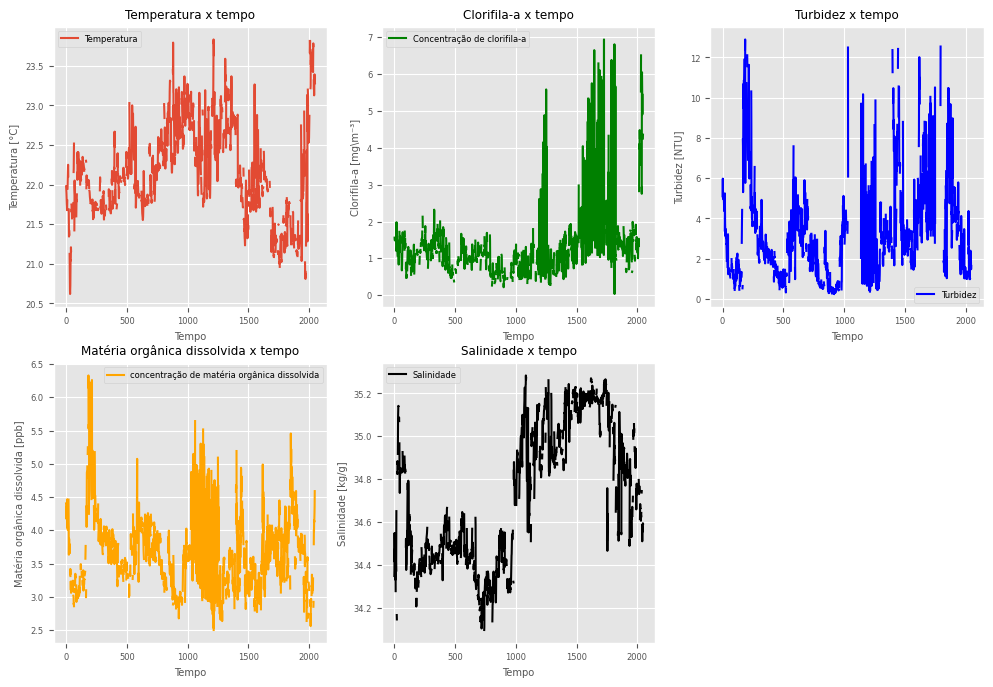
\includegraphics[width=1\linewidth]{lista1-1b}
	\caption{Variáveis disponível no dado do SIMCOSTA}
	\label{fig:lista1-1b}
\end{figure}
	Conforme se observa na figura \ref{fig:lista1-1b}, existe a necessidade de interpolação dos dados, pois existem lacunas nos mesmos.
	
\begin{figure}[H]
	\centering
	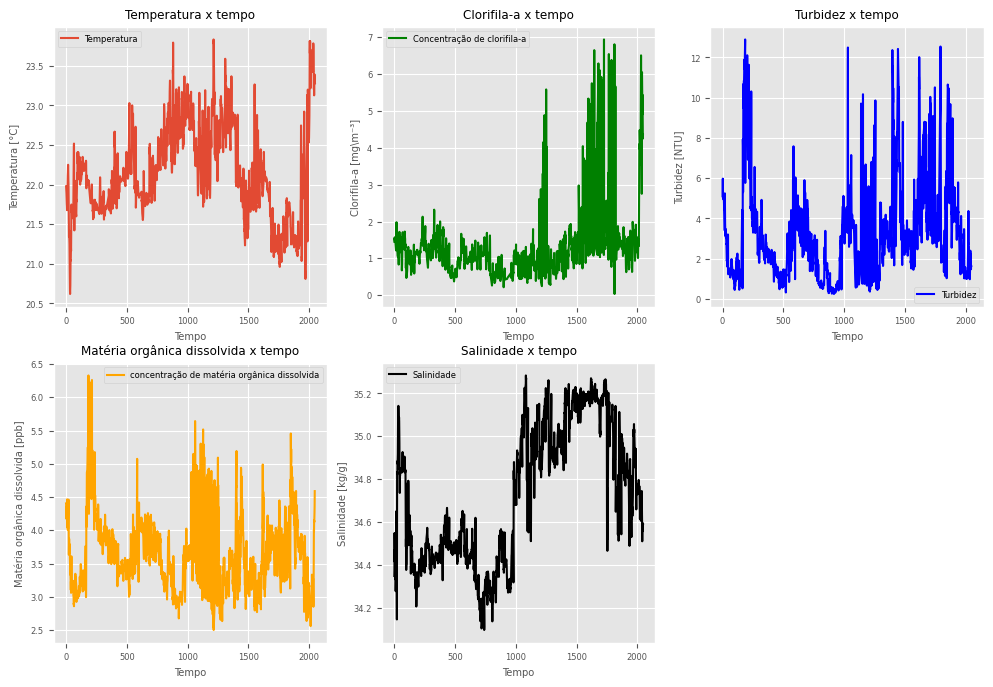
\includegraphics[width=1\linewidth]{lista1-1c}
	\caption{Variáveis disponível no dado do SIMCOSTA após interpolação linear}
	\label{fig:lista1-1c}
\end{figure}
	A figura \ref{fig:lista1-1c} mostra os dados após uma interpolação linear utilizando o pacote pandas do Python.
	\begin{python}
pandas.DataFrame.interpolate
	\end{python}
	
	É notável que mesmo após a interpolação os dados apresentam pontos que não representam o comportamento da série e podem ter ocorrido devido a algum erro/processo que não seja do interesse. Com isso surge a necessidade da utilização de uma edição na série temporal.
	
	Utilizando o \textit{wild edit}, foi realizada a edição dos dados como pode ser visto na figura \ref{fig:lista1-2i}
\begin{figure}[H]
	\centering
	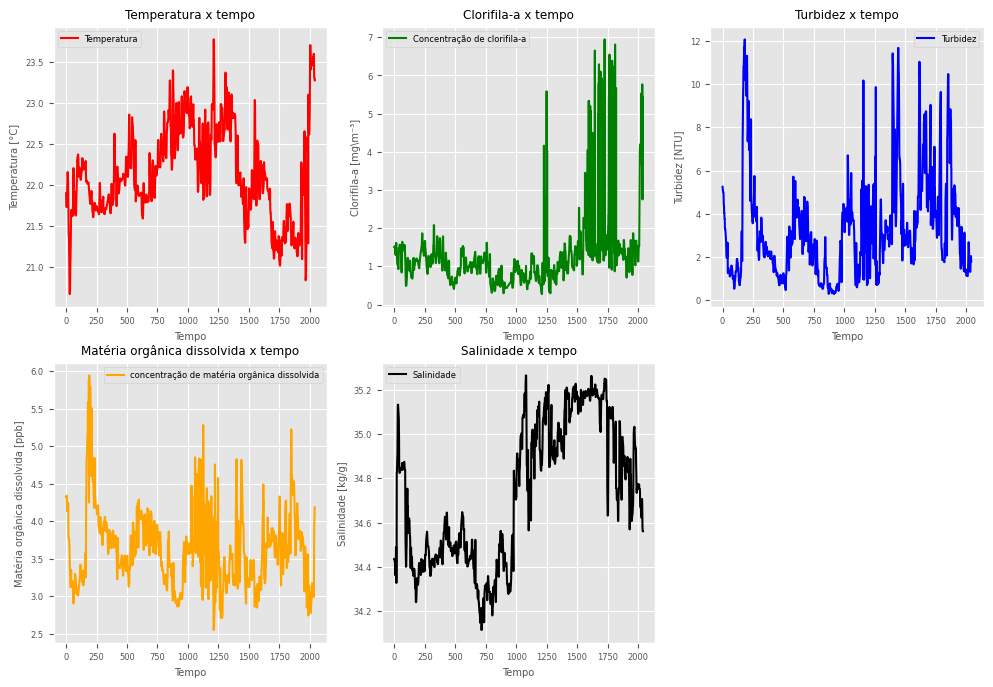
\includegraphics[width=1\linewidth]{lista1-2i}
	\caption{Variáveis editadas pelo conceito de \textit{wild edit}}
	\label{fig:lista1-2i}
\end{figure}
	
	Os \textit{spikes} foram removidos de forma que a série temporal original não seja muito afetada, com esse método funcionando com uma especie de janelamento dos dados, a figura \ref{fig:lista1-2} mostra uma comparação dos dados originais com os editados para a salinidade, onde é visível que o padrão da série se mantem com apenas os \textit{spikes} sendo removidos, esse método pode induzir a erros que não facilmente detectáveis devido a forma que ele é feito. Dependendo da analise a ser realizada, outras edições ou diferentes métodos possam ser necessários.

\begin{figure}[H]
	\centering
	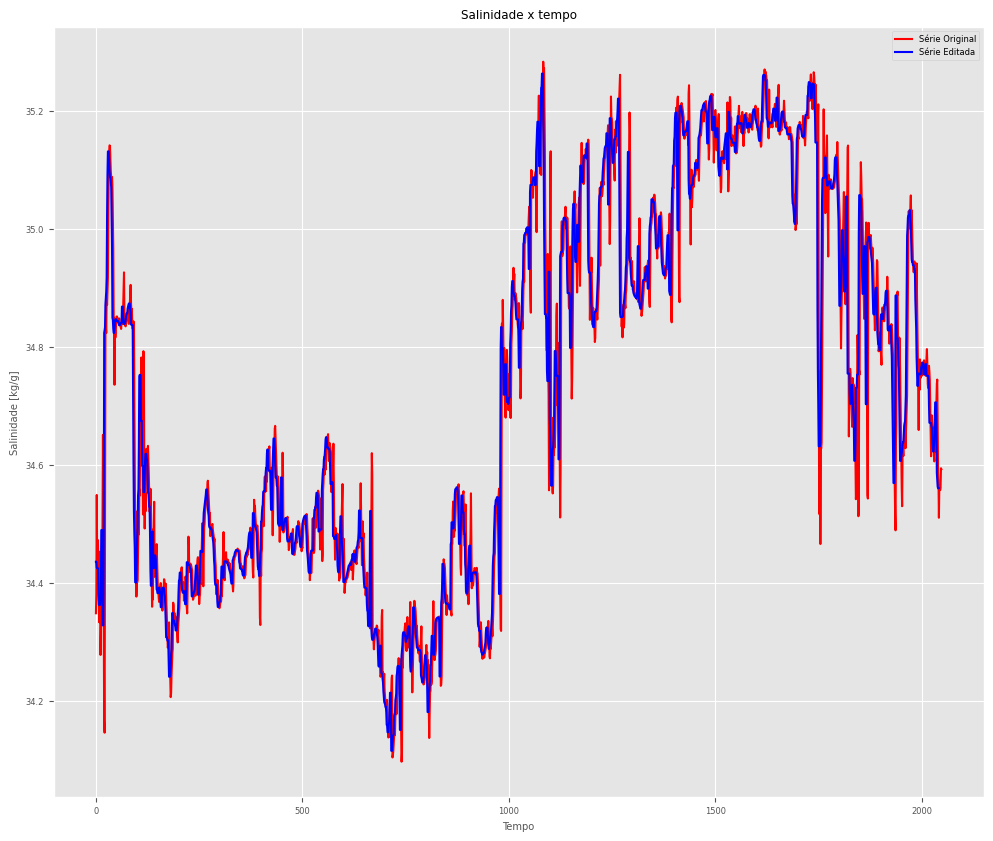
\includegraphics[width=0.8\linewidth]{lista1-2}
	\caption{Comparação da salinidade sem edição e com edição}
	\label{fig:lista1-2}
\end{figure}
	\newpage
	\textbf{Parte II – Estatística básica}
	
\begin{figure}[H]
	\centering
	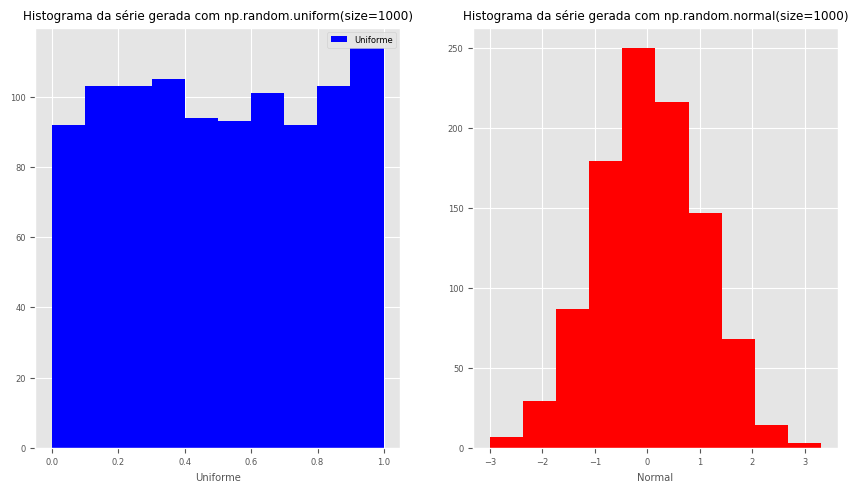
\includegraphics[width=0.99\linewidth]{lista1-3a}
	\caption{Histograma de funções aleatórias geradas com o modo uniforme e normal respectivamente}
	\label{fig:lista1-3a}
\end{figure}
	
	\begin{table}[H]
\centering

	\begin{tabular}{|c|c|c|}
		\hline
		& Média & Desvio Padrão \\
		\hline
		Uniforme & 0.506 & 0.291 \\
		\hline
		Normal & 0.035 & 0.98 \\
		\hline
	\end{tabular}
	\caption{Média e desvio padrão para cada série aleatória}
		\end{table}
Devido a forma que as distribuições estatísticas são calculadas, os valores de média e desvio padrão estão dentro do esperados.  \\

Para um sinal aleatório com distribuição normal com média de 14.7 e desvio padrão de 4.7, se pode utilizar a função da biblioteca NumPy para Python:
\begin{python}
temprand = np.random.normal(loc=14.2,scale=4.7,size=10000)
\end{python}
Com isso se pode calcular o z-score com o pacote SciPy:
\begin{python}
zscores = stats.zscore(temprand)
\end{python}
A média e o desvio padrão do z-score é apresentado na tabela \ref{szsoretab}
	\begin{table}[H]
	\centering
\begin{tabular}{|c|c|}
	\hline
	Média & Desvio Padrão \\
	\hline
	0 & 1 \\
	\hline
\end{tabular}

\caption{Média e desvio padrão do z-score}
\label{szsoretab}
\end{table}

A figura \ref{fig:lista1-3} apresenta o histograma do z-score
\begin{figure}[H]
	\centering
	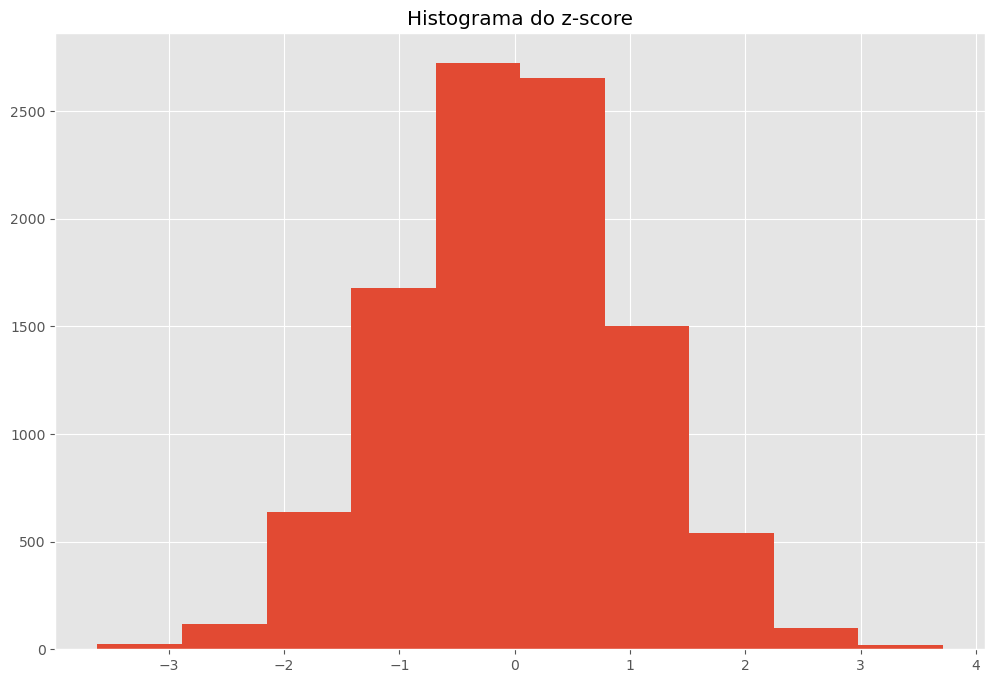
\includegraphics[width=0.9\linewidth]{lista1-3.2c}
	\caption{Histograma do z-score para uma função aleatória normal}
\label{fig:lista1-3}
\end{figure}
Com os resultados apresentando o comportamento esperado para a padronização realizada. O gráfico de probabilidade pode ser feito utilizando a função:
\begin{python}
probplot = stats.probplot(zscores, plot=plt)
\end{python}
	
\begin{figure}[H]
	\centering
	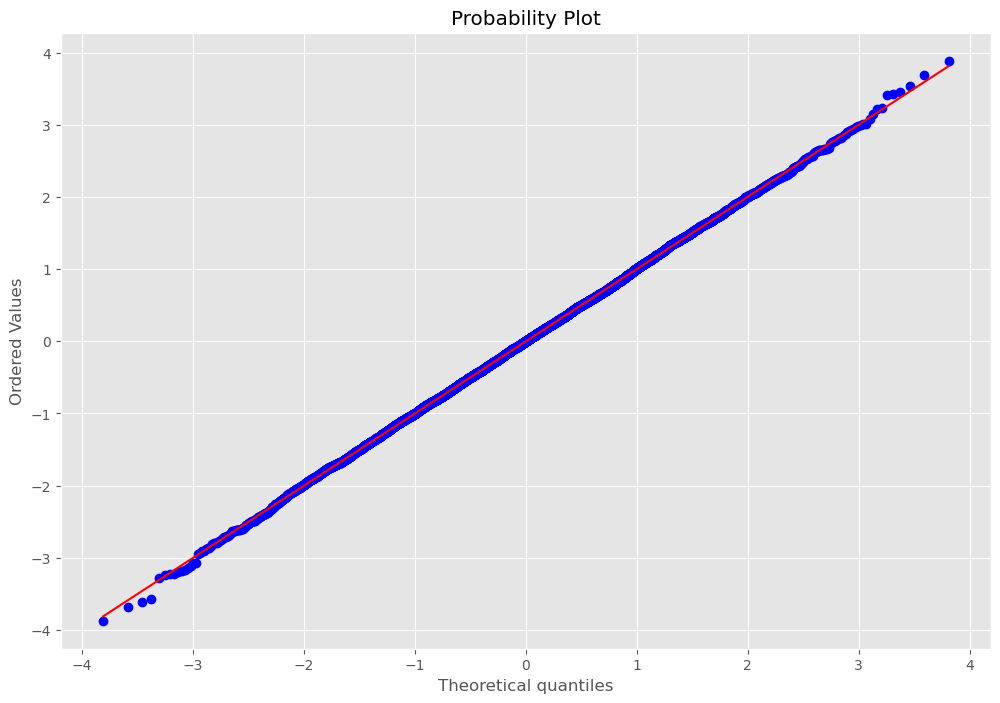
\includegraphics[width=0.9\linewidth]{lista1-3.2d}
	\caption{Gráfico de probabilidade normal da série}
	\label{lista1-3.2d}
\end{figure}
Pela figura \ref{lista1-3.2d}, se observa que os dados gerados aleatoriamente e normalizados utilizando o z-score seguem a distribuição normal, com praticamente todos os pontos próximos a linha de regressão. \\

A função de densidade de probabilidade normal da série $x$ variando de 0 a 30 pode ser calculada com:
\begin{python}
a30 = np.arange(start=0,stop=30,step=0.1)
a30pdf=stats.norm.pdf(a30,14.2,4.7)
\end{python}
Onde a função stats.\textcolor{cyan}{norm}.pdf() calcula a densidade de probabilidade normal de $x$ variando entre 0 e 30 com intervalo 0.1
\begin{figure}[H]
	\centering
	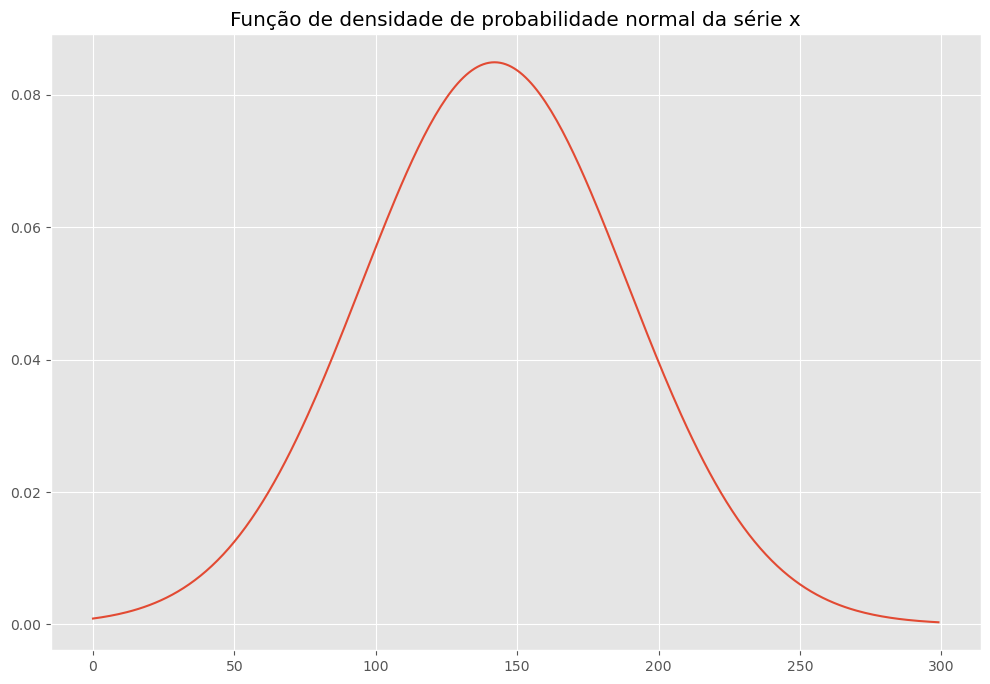
\includegraphics[width=0.9\linewidth]{lista1-3.3c}
	\caption{Função de densidade de probabilidade normal da série x}
	\label{fig:lista1-3.3c}
\end{figure}
O z-score será calculada da mesma forma, com os resultados para a média e desvio apresentados na tabela \ref*{szsorea30}

			\begin{table}[H]
			\centering
			\begin{tabular}{|c|c|}
				\hline
				Média & Desvio Padrão \\
				\hline
				0 & 1 \\
				\hline
			\end{tabular}
			
			\caption{Média e desvio padrão do z-score da função de densidade de probabilidade normal}
			\label{szsorea30}
		\end{table}	
		
\begin{figure}[H]
	\centering
	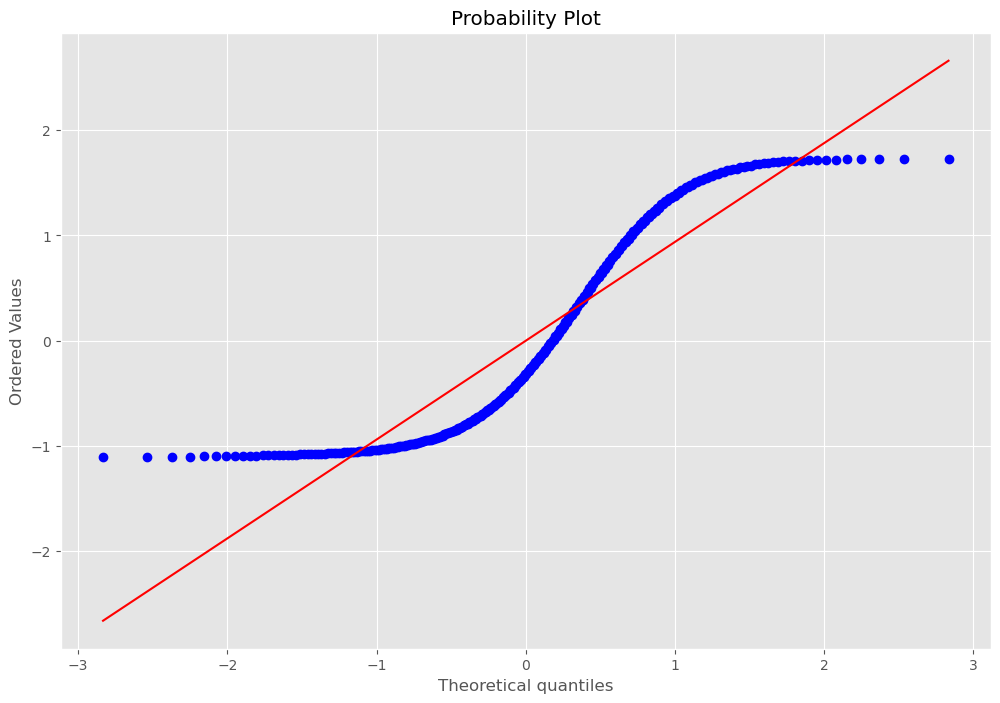
\includegraphics[width=0.9\linewidth]{lista1-3.3d}
	\caption{Gráfico de probabilidade normal da série}
	\label{lista1-3.3d}
\end{figure}
Pela figura \ref{lista1-3.3d} é possível ver que embora exista um padrão na orientação dos pontos com a linha de regressão, eles aparatam ter um comportamento não-linear em relação com a probabilidade normal, indicando que não seguem totalmente a distribuição normal. 

O valor acumulado da probabilidade normal da série $x$ variando de 0 a 30 pode ser calculada com:
\begin{python}
	a30cdf=stats.norm.cdf(a30,14.2,4.7)
\end{python}
\begin{figure}[H]
	\centering
	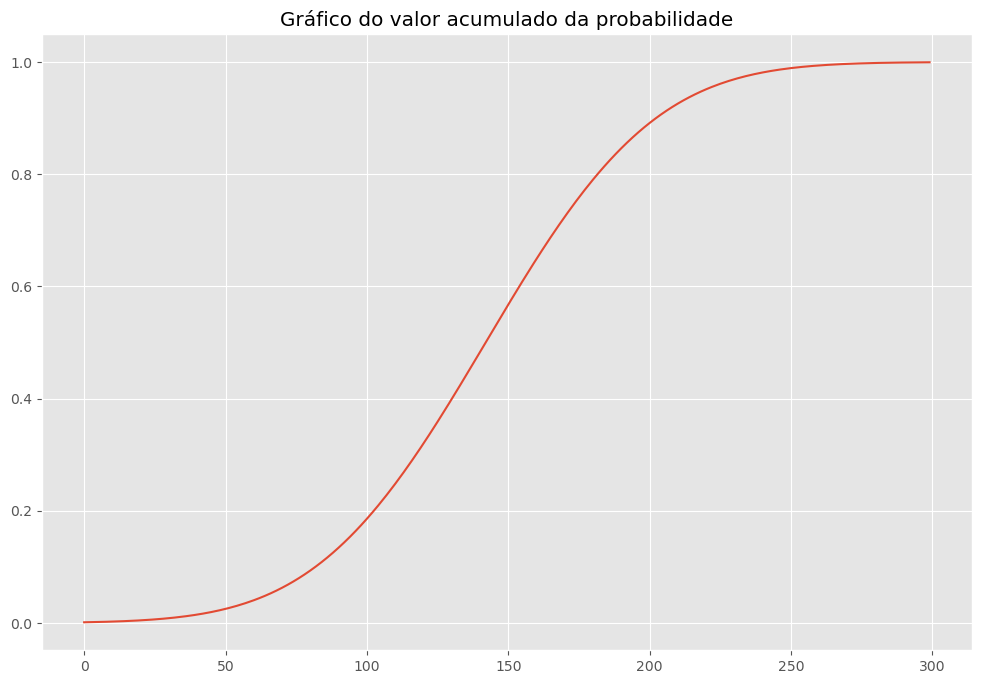
\includegraphics[width=0.9\linewidth]{lista1-3.3f}
	\caption{Gráfico do valor acumulado da probabilidade}
	\label{fig:lista1-3.3f}
\end{figure}
A probabilidade de encontrar um valor de $x\leq 3$ é de 0.851\% já para um valor de $x\geq 20$ é de 10.85\%. 

Utilizando a função:
\begin{python}
_,pvalue=sm.lilliefors(a30pdf,dist='norm')
\end{python}
Se obtém um valor de 0.001, ou seja, a hipótese nula não pode ser rejeitada e os dados são originários de uma distribuição normal.


\end{document}